\chapter{Description of the early packages used in simulation}
\label{sec:earlyPackages}

At the beginning of the project, were created some ROS packages so as to obtain the necessary experience and get familiar with the system. Furthermore, possibly dangerous or unpredicted situations in the real system were avoided by carefully studying the MAV's simulated responses to the experiments. All the following packages were written on a computer running on Ubuntu 14.04 LTS alongside with ROS Indigo Igloo. The simulator used in this project is Gazebo\cite{GazeboSimulator} as provided by ROS. Now follows the description of the ROS packets, some packets with very similar role and structure are omitted from the description. All the aforementioned packages are written in the C\texttt{++} programming language\cite{Stroustrup} and can be accessed at the ASL's GitHub page under the repository mav\textunderscore demos\cite{MyRepoGitHub}. 


\section{Connecting the Camera with ROS}
\label{sec:connectedCamera}
The very first task was to connect a camera to the ROS so as to obtain the images of the markers. The camera chosen for this project was the Logitech Tessar HD, for its calibration and image rectification the ROS camera\textunderscore calibration package and the image \textunderscore proc node were used respectively. After the camera setup, the detection of the Apriltags\cite{olson2011tags} came into focus. In order to detect the position and orientation of the aforementioned, the apriltag\textunderscore ros package was used. This provides a ROS wrapper for the C\texttt{++} library\cite{ROSApriltag}. An example of such a tag is provided in figure \ref{pics:tag36h11}. It should be mentioned that although this library detects distance and yaw accurately it faces some problems with the detection of the marker's roll and pitch angles.

\begin{figure}
   \centering
   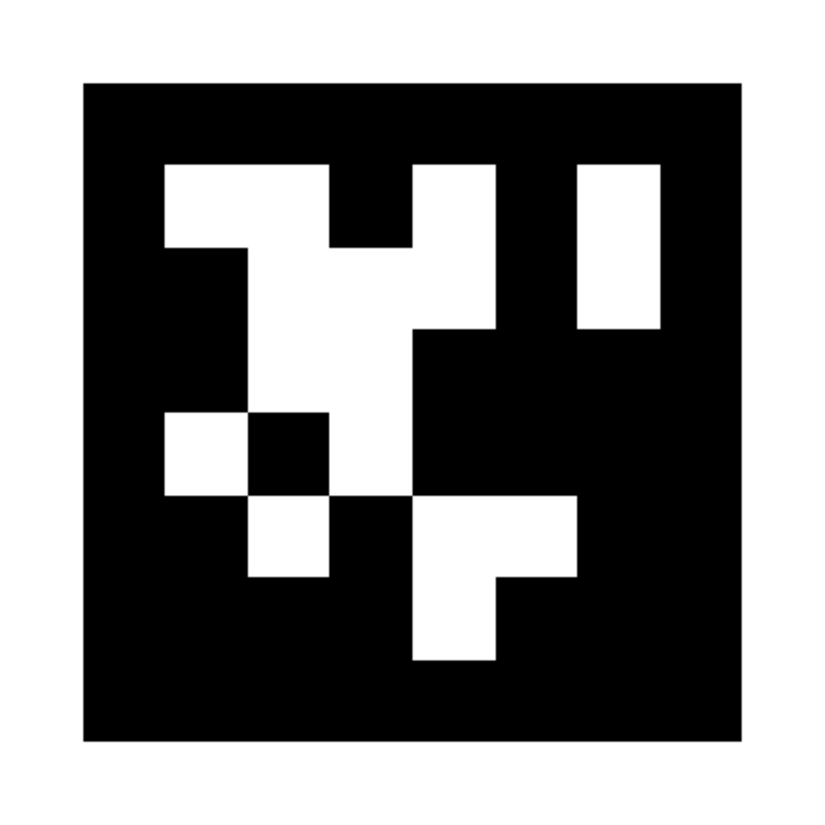
\includegraphics[width=0.55\textwidth]{images/tag36h11_im_large.pdf}
   \caption{Ein Bild}
   \label{pics:tag36h11}
\end{figure}


\section{Moving the Simulated MAV}
\label{sec:movingMAV}
After the camera setup, the main focus moved towards connecting the camera image with simulated MAV. This was conducted in the mav\textunderscore demo\textunderscore camera package. In there two nodes are created, except of course those referring to camera, one that detects the Apriltag and publishes the detection data to a ROS topic and another one that conducts the motion. In this specific example the user moves the tag in front of the camera and the simulated MAV moves accordingly. As can be seen from figure \ref{pics:mav_demo_camera} when the package is ran, two windows are created, one depicting the detected apriltag, for the user to know whether or not the marker is detected and the simulator's window with the moving MAV. In figure \ref{pics:mav_demo_camera_rosgraph} are depicted all the ROS running nodes. 

For safety reasons, the position of the MAV in the z axis is augmented by 50 cm. 
Thus, when the user holds the marker at the same height as the camera, the MAV does not collide with the floor.

\begin{figure}
   \centering
   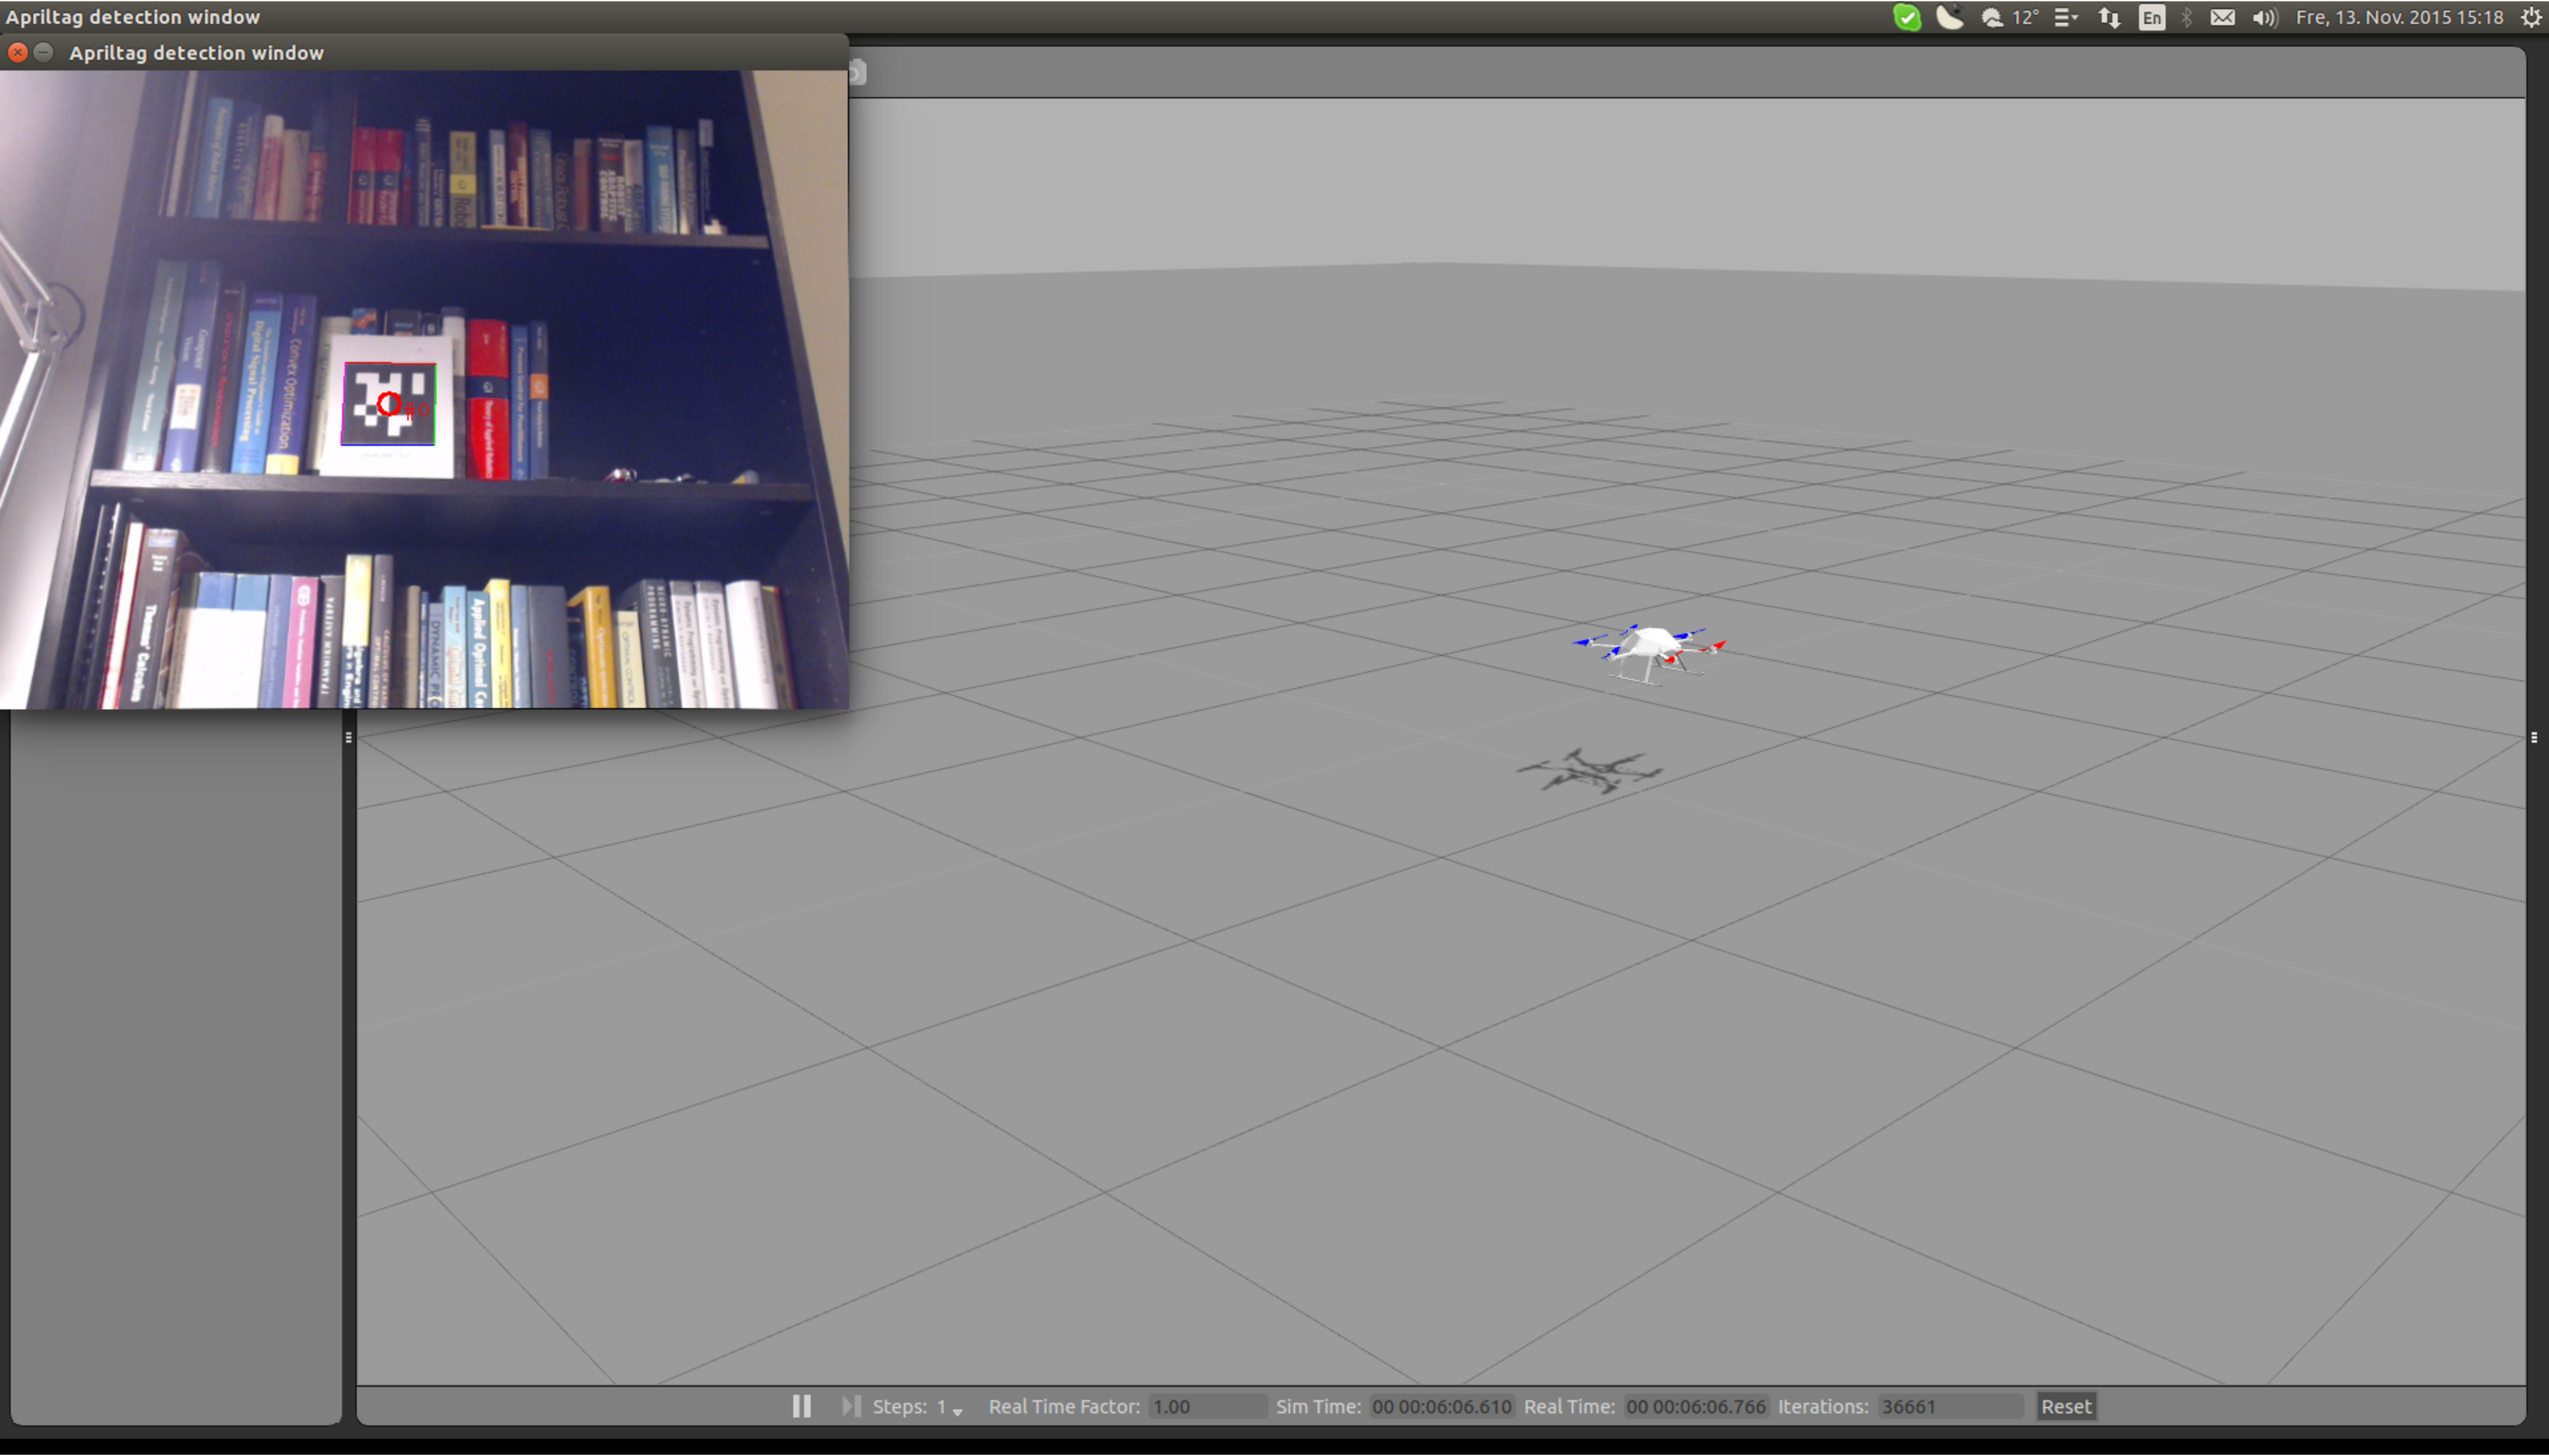
\includegraphics[width=0.75\textwidth]{images/mav_demo_camera.pdf}
   \caption{Ein Bild}
   \label{pics:mav_demo_camera}
\end{figure}

\begin{figure}
   \centering
   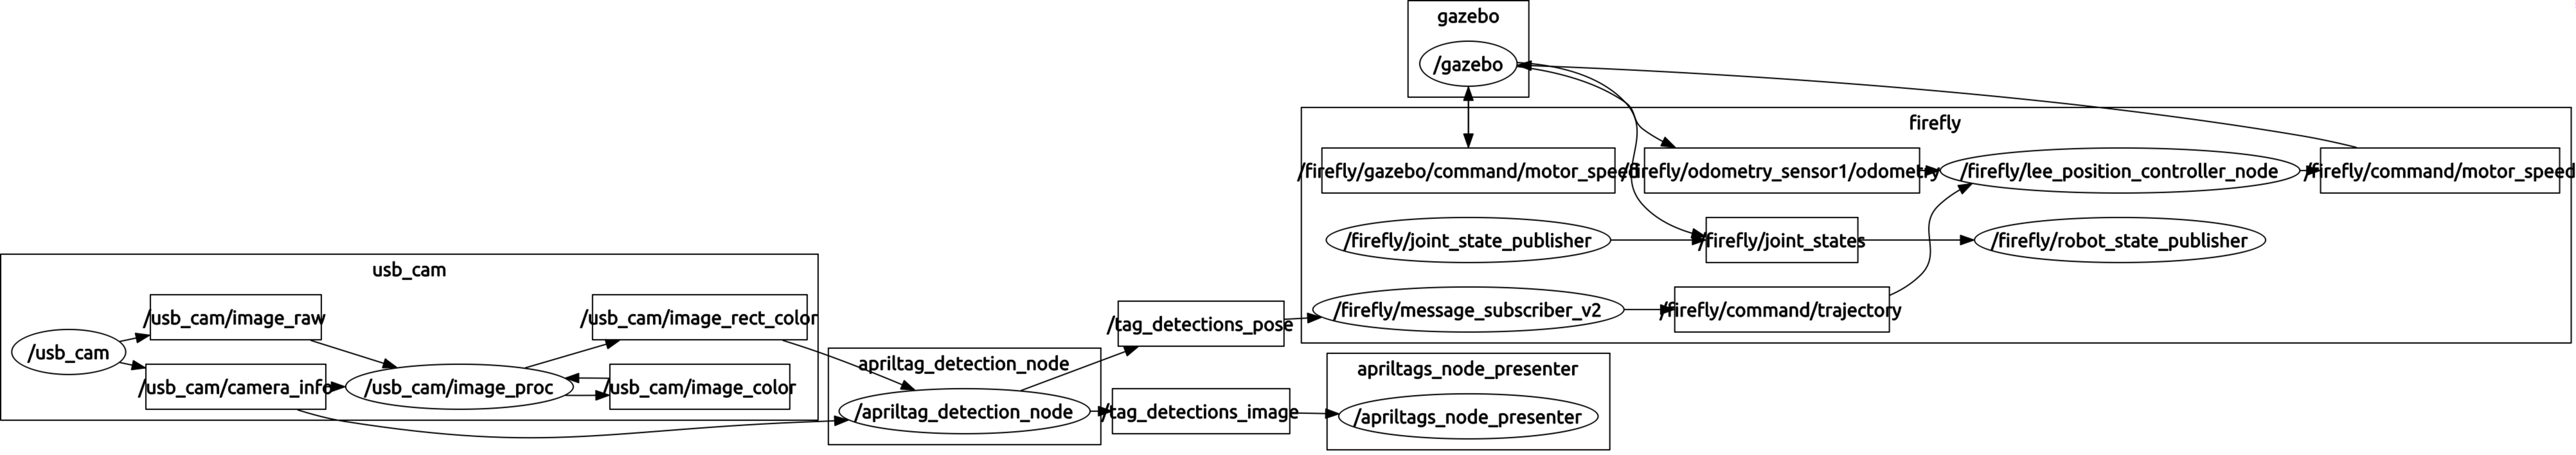
\includegraphics[width=0.98\textwidth]{images/mav_demo_camera_rosgraph.pdf}
   \caption{Ein Bild}
   \label{pics:mav_demo_camera_rosgraph}
\end{figure}

\section{Creating the Apriltag Models}
\label{sec:cubeRobots}

In order to make the simulation realistic, the MAV should detect the Apriltags by its own camera. Thus, models represented the various tags were needed. The objects were simple cuboids which had as texture the Apriltag's image. It should be mentioned that the dimensions (width and height) of the cuboids should be identical as the parameters passed from the ROS parameter server to the detection node, so as to get the correct distance estimation. 

\section{Realistic Simulation Scenarios}
\label{sec: apriltagFireflySimulation}

Before moving to the real system, were implemented some more realistic simulation scenarios so as to study the MAV's behavior under various circumstances. In this case the user inserts different markers inside the simulated world and the MAV performs a variety of motions with respect to the different markers it detects from its own camera. In order to perform different motions the MAV detects the id of each tag, and executes the predefined motions. It should be mentioned, that at each time only one Apriltag should be detected from the MAV's sensor so as to have a smooth operation.

The default motion, consists of the user moving a marker in front of the computer's camera which controls the pose of the Apriltag in the simulation. The MAV is programmed to follow the marker, by having adequate distance so as to guarantee the user's safety in the real world system. The predefined safety distance is set by the user at the launch of the simulation, in the case that the user enters a values less than a predefined threshold, the program automatically sets the input value to the threshold. When the user rotates the marker in the z axis (yaw) by $\psi$ degrees the MAV performs a circle-like motion with respect to the marker's position. 

Furthermore, the MAV is capable of performing take-offs and landings whenever the user wants. When the user wants to land the MAV, he just has to present a specific marker in front of the camera. The exact same procedure, but with a different marker, is followed for making the MAV hovering again. The program stores the last x,y coordinates of The MAV before the landing command and automatically sets the desired height at 1m. 

//Depending on the implementation //Right now square    





















  